\documentclass[10pt]{article}
\usepackage[ngerman]{babel}
\usepackage[utf8]{inputenc}
\usepackage[T1]{fontenc}
\usepackage{amsmath}
\usepackage{amsfonts}
\usepackage{amssymb}
\usepackage[version=4]{mhchem}
\usepackage{stmaryrd}
\usepackage{graphicx}
\usepackage[export]{adjustbox}
\graphicspath{ {./images/} }
\usepackage{bbold}

\title{Hauptprüfung Abiturprüfung 2021 - Leistungsfach }

\author{Alexander Schwarz\\
www.mathe-aufgaben.com}
\date{}


\begin{document}
\maketitle
 Baden-WürttembergAugust 2021

\section*{Aufgabe B2}
Eine Firma stellt Gewächshäuser her. Die Ecken der Grundfläche dieser Gewächshäuser können modellhaft durch die Punkte $\mathrm{A}(8|0| 0), \mathrm{B}(8|7| 0), \mathrm{C}(0|7| 0)$ und $\mathrm{D}(0|0| 0)$ beschrieben werden. In diesen Ecken stehen senkrecht zur Grundfläche Pfosten, die das Dach des Gewächshauses tragen (alle Koordinatenangaben in Meter).\\
a) Bei einem dieser Gewächshäuser können die Ecken der Dachfläche durch die Punkte $\mathrm{E}(8|0| 4), \mathrm{F}(8|7| 5), \mathrm{G}(0|7| 5)$ und $\mathrm{H}(0|0| 4)$ beschrieben werden. Stellen Sie dieses Gewächshaus in einem geeigneten Koordinatensystem dar. (1 VP)

Berechnen Sie den Rauminhalt dieses Gewächshauses.\\
Ermitteln Sie eine Koordinatengleichung der Ebene, die die Lage der Dachfläche beschreibt.\\
b) Die Firma bietet die Gewächshäuser mit unterschiedlichen Neigungen der Dachfläche an. Die Lage jeder dieser Dachflächen kann durch eine Ebene beschrieben werden, die zur Schar $\mathrm{E}_{\mathrm{a}}: \mathrm{ax}_{2}-7 \mathrm{x}_{3}=7 \mathrm{a}-35$ mit $\mathrm{a} \geq 0$ gehört.

Berechnen Sie den Wert von a, für den die Neigung der Dachfläche $30^{\circ}$ beträgt. (2 VP)\\
Es gibt eine Gerade g, die in allen Ebenen der Ebenenschar liegt. Bestimmen Sie eine Gleichung dieser Geraden g.

Untersuchen Sie, für welche Werte von a im gesamten Gewächshaus eine Mindesthöhe von 2 m gegeben ist.\\
(2 VP)

\section*{Lösungen}
\section*{Aufgabe B2}
a) Stellen Sie dieses Gewächshaus in einem geeigneten Koordinatensystem dar.\\
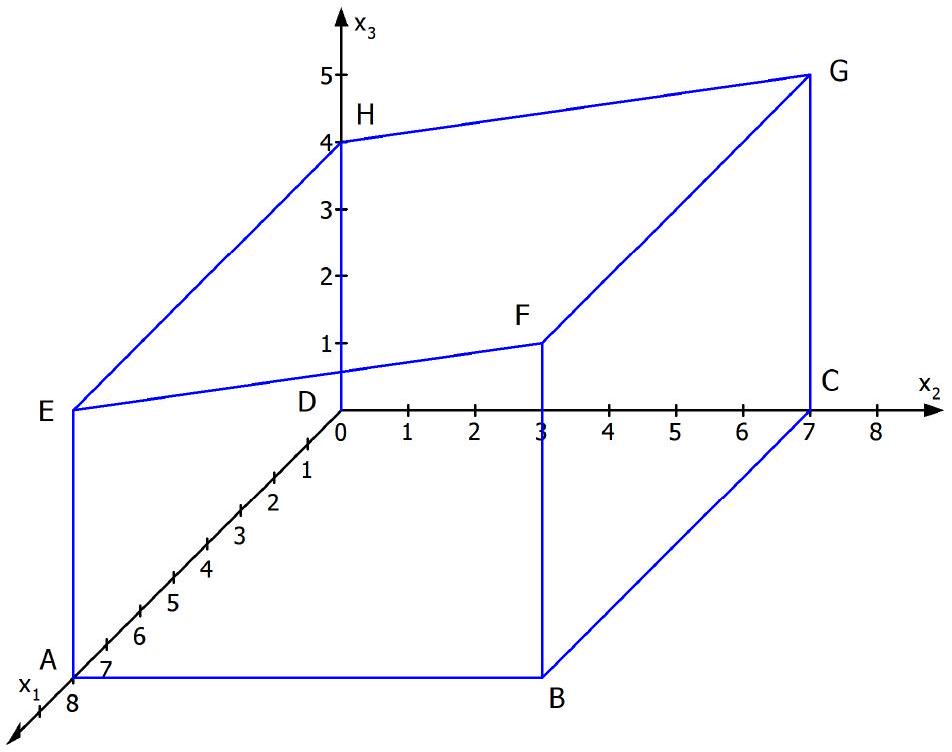
\includegraphics[max width=\textwidth, center]{2025_04_24_20733abc36550fde66fag-3}

Berechnen Sie den Rauminhalt dieses Gewächshauses.\\
Volumen $=\mathrm{G} \cdot \mathrm{h}$\\
G = Grundfläche $=$ Trapezfläche $A B E F=\frac{4+5}{2} \cdot 7=31,5 \mathrm{~m}^{2}$\\
h = Höhe des Prismas = 8\\
$V=31,5 m^{2} \cdot 8 m=252 m^{3}$

Ermitteln Sie eine Koordinatengleichung der Ebene, die die Lage der Dachfläche beschreibt.\\
Parameterform der Ebene K durch die Punkte E, F, G: $\vec{x}=\left(\begin{array}{l}8 \\ 0 \\ 4\end{array}\right)+r \cdot\left(\begin{array}{l}0 \\ 7 \\ 1\end{array}\right)+s \cdot\left(\begin{array}{c}-8 \\ 7 \\ 1\end{array}\right)$\\
Normalenvektor der Ebene K: $\overrightarrow{\mathrm{n}}=\left(\begin{array}{l}0 \\ 7 \\ 1\end{array}\right) \times\left(\begin{array}{c}-8 \\ 7 \\ 1\end{array}\right)=\left(\begin{array}{c}0 \\ -8 \\ 56\end{array}\right)$ bzw. $\overrightarrow{\mathrm{n}}^{*}=\left(\begin{array}{c}0 \\ -1 \\ 7\end{array}\right)$\\
Ansatz für die Koordinatengleichung: $\mathrm{K}:-\mathrm{x}_{2}+7 \mathrm{x}_{3}=\mathrm{d}$\\
Einsetzen des Punktes $G(0|7| 5): d=28$\\
Koordinatengleichung: K: $-\mathrm{x}_{2}+7 \mathrm{x}_{3}=28$\\
b) Berechnen Sie den Wert von a, für den die Neigung der Dachfläche $30^{\circ}$ beträgt.

Der Neigungswinkel entspricht dem Schnittwinkel einer Scharebene $\mathrm{E}_{\mathrm{a}}$ mit der $\mathrm{x}_{1}-\mathrm{x}_{2}$-Ebene.\\
$\cos 30^{\circ}=\frac{\left|\left(\begin{array}{c}0 \\ a \\ -7\end{array}\right) \cdot\left(\begin{array}{l}0 \\ 0 \\ 1\end{array}\right)\right|}{\sqrt{a^{2}+49} \cdot \sqrt{1}} \quad \Leftrightarrow \frac{1}{2} \sqrt{3}=\frac{7}{\sqrt{a^{2}+49}}$\\
$\left.\Leftrightarrow \sqrt{\mathrm{a}^{2}+49}=\frac{14}{\sqrt{3}} \quad \right\rvert\,$ quadrieren\\
$\Rightarrow \mathrm{a}^{2}+49=\frac{196}{3} \Leftrightarrow \mathrm{a}^{2}=\frac{49}{3} \quad \Rightarrow \mathrm{a}= \pm \sqrt{\frac{49}{3}}$\\
Wegen $\mathrm{a} \geq 0$ kommt nur $\mathrm{a}=\sqrt{\frac{49}{3}}$ in Betracht.

Bestimmen Sie eine Gleichung dieser Geraden g.\\
Wähle zwei beliebige Ebenen der Schar aus (z.B. für $a=0$ und $a=1$ ) und bestimme die Schnittgerade dieser Ebenen:\\
$E_{0}:-7 x_{3}=-35$\\
$\mathrm{E}_{1}: \mathrm{x}_{2}-7 \mathrm{x}_{3}=-28$\\
Lösung des Gleichungssystems:\\
Aus der 1.Zeile folgt $x_{3}=5$\\
Aus der 2.Zeile folgt $x_{2}-35=-28 \Leftrightarrow x_{2}=7$\\
Außerdem gilt $\mathrm{x}_{1}=\mathrm{t}$ mit $\mathrm{t} \in \mathbb{R}$, da das Gleichungssystem nicht die Variable $\mathrm{x}_{1}$ enthält und diese damit einen beliebigen Wert annehmen kann.

Aus den Lösungen ergibt sich die Schnittgerade: $g: \vec{x}=\left(\begin{array}{l}0 \\ 7 \\ 5\end{array}\right)+t \cdot\left(\begin{array}{l}1 \\ 0 \\ 0\end{array}\right)$.\\
Hinweis:\\
Bei dieser Aufgabe muss nicht überprüft werden, ob die Gerade g auch auf allen anderen Ebenen der Schar liegt, da in der Aufgabenstellung formuliert ist, dass es solch eine Gerade g gibt.

Untersuchen Sie, für welche Werte von a im gesamten Gewächshaus eine Mindesthöhe von $2 m$ gegeben ist.

Die Wand, die durch das Rechteck BCGF dargestellt wird, hat eine Höhe von 5 Metern und diese Höhe bleibt für alle Werte von a gleich.\\
Begründung: Die Gerade g, durch die alle Ebenen der Schar gehen enthält die Punkte F und G des Gewächshauses.

Der Spurpunkt einer beliebigen Scharebene mit der $x_{3}$-Achse ist $H_{a}(0|0| 5-a)$. Der Term 5 - a stellt die Höhe der Wand dar, die der Wand BCGF gegenüber liegt.\\
Es muss also gelten: $5-\mathrm{a} \geq 2$ und damit $\mathrm{a} \leq 3$ und aufgrund der Bedingung in der Aufgabe a $\geq 0$.\\
Insgesamt muss $0 \leq a \leq 3$ sein.


\end{document}